\section{Results}\label{sec:results}

With a complete experimental set-up, benchmark performance was established using the simple models ranging from the
SVM to the basic fully-connected network, at around 70-80\%.
Both 2 dimensional and 3 dimensional convolutional networks were able to surpass the benchmarks,
attaining 95\%+ accuracy.

The stretch goal of region highlighting using unsupervised segmentation proved infeasible for this project timeframe, given
the challenges overcome with the 3d convolutional model architecture.

\subsection{Model Architecture}\label{subsec:model-arch}

I explored the available hyperparameters of the chosen model architectures to a minor degree, focusing on
establishing optimal learning rates with the chosen optimizer and model, with the given normalized data.

Typically 1e-2 to 1e-4 worked, with learning rates on the order of 1e-3 being best for both ResNet style convolutional
networks.

Stochastic Gradient Descent with nesterov momentum on Cross Entropy Loss performed very well.
Other optimizers like Adam and loss metrics like NLL Loss explored were either on par or worse and thus not
further utilized.

None of my attempted customizations to the ResNet architecture netted any improvements, including expanding filter sizes
or adding normalization layers.

\subsection{Subject individuality}\label{subsec:subjects-individ}

Interestingly, performance of models on subjects not included in the training run was subpar.
For example, a model trained to 95\% accuracy on 6 subjects alone would fair closer to 60\% on 6 new subjects.
I speculate this is not overly worrisome, and a consequence of using such a small handful of subjects.
Better generalizability seems likely given an investment in much larger machinery or methodology capable of handling
more subjects, or better normalization practices.
One exploration of the data revealed by far most of the variance comes at the perimeter of the cortex suggesting slightly
varied sizes of brains not overlapping perfectly.
Convolutional networks should be able to tackle this dilemma with no problem but perhaps the small dataset makes
spatial and orientation noise more consequential.

\subsection{Training Progress}\label{subsec:training-prog}

Generally, training catches within about 20 epochs, learning to differentiate better than chance on 2
dimensional data~\ref{fig:2d_cold}, taking noticeably longer for 3 dimensional data~\ref{fig:3d_cold} to catch up,
as there's presumably more nuance to learn.
The learning rate may seem fairly aggressive~\ref{fig:cold_500_loss.png}
and takes one step back for every two steps forward, but overall produces
more competitive results than a gentler learning rate.

 \begin{figure}
  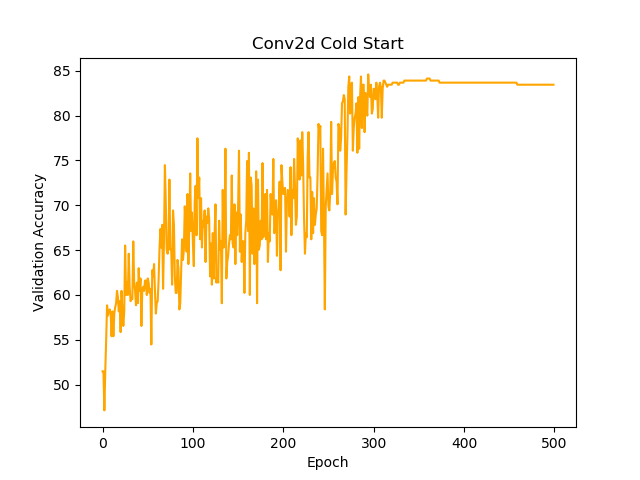
\includegraphics[width=\linewidth]{images/2d_cold.png}
  \caption{Cold-Start 2D Training Progress}
  \label{fig:2d_cold}
\end{figure}

 \begin{figure}
  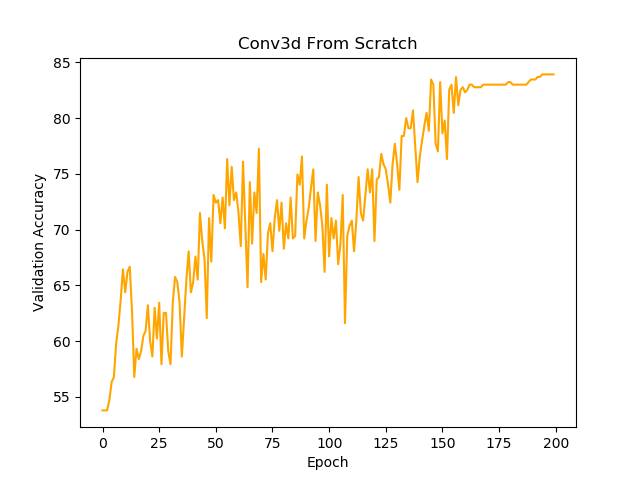
\includegraphics[width=\linewidth]{images/3d_cold.png}
  \caption{Cold-Start 3D Training Progress}
  \label{fig:3d_cold}
\end{figure}

 \begin{figure}
  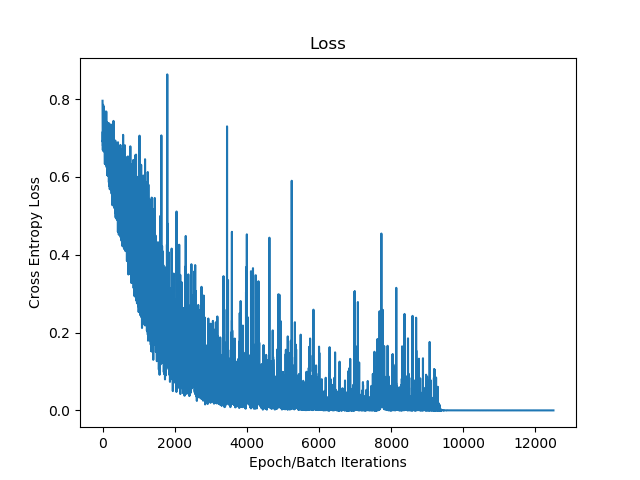
\includegraphics[width=\linewidth]{images/cold_500_loss.png}
  \caption{Cold-Start Training Progress Loss}
  \label{fig:cold_500_loss.png}
\end{figure}

\subsection{Warm Starts}\label{subsec:warm-starts}

Saving the model parameters and training again on a new subset of subjects or even resuming learning
on the same division worked wonderfully.

Getting the model to a stable, low 80\% performance leaves us in an excellent place to begin aggressively learning again.

With this method performances of over 95\%~\ref{fig:2d_warm} are common.

As mentioned before however, higher performances are typically seen on the same subject, though it doesn't take
long for the model to adapt to the new group of subjects for training, but of course it sacrifices performance on the
previous grouping to do so.

 \begin{figure}
  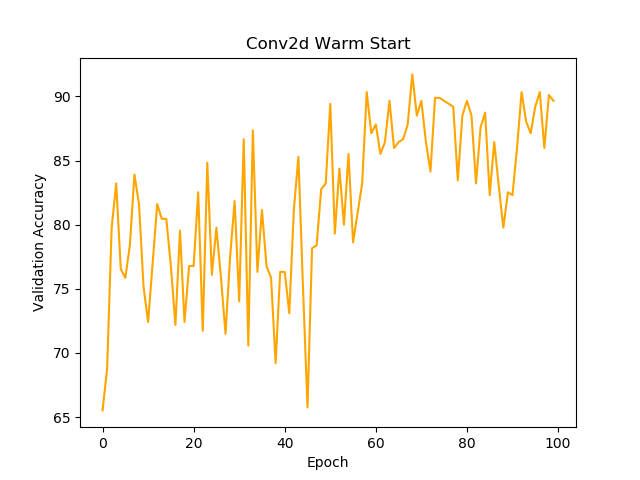
\includegraphics[width=\linewidth]{images/2d_warm.png}
  \caption{Warm-Start 2D Training Progress}
  \label{fig:2d_warm}
\end{figure}

\subsection{3 Dimensions}\label{subsec:3-dimensions}

One of the biggest challenges of this endeavor has been coping with the computational demands that the third
dimension adds.
Video data is notoriously large, and now I've seen 3d CNN's can be as well.
Our application here substitutes time for a third spatial axis, and does seem to be a richer dataset to draw from for
classification.
Training on a larger, more complex dataset does feel more challenging as well, with training taking longer to catch on
to something productive.

Unfortunately, I've found iterating with 3 dimensional models to be much harder than 2d which makes refinement also a
bit of a challenge.
Where training may take 15 minutes with a 2d CNN, it might be 5 hours or more with a 3d CNN, and the limitations on the
quality and abundance of the dataset size kick in much faster than for 2d.
The dataset is already a fairly conservative low-grade rendering of the brain and aggresive interpolation cuts into
performance directly.
Additionally, lowering the batch size is very detrimental to performance, with at least 64 images being critical to
learning generalizable patterns at each step in an epoch.
However, what I have seen in working with the 3d CNN's is that they are very performant, achieving on par or
3 to 4\% higher classification accuracy compared to their 2d counterparts, and responding encouragingly as well to warm-starts,
to which I'm very pleased.

\subsection{Performance Measures}\label{subsec:performance}

Here I examine one highly performant 2d convolutional network in more detail.
Thankfully it is a well balanced model, with seemingly high intuitive understanding of the differentiable characteristics
of brain activity, as it's highly accurate, and highly confident in it's decisions.

While I have been able to tweak the model to exceed this accuracy, this is in my opinion the most balanced
run observed as typically the model begins to favor performance on one class over the other despite near
equal representation.

 % P-R-F1-S
\begin{center}
 \begin{tabular}{||c c c||}
 \hline
 - & Nonfood & Food \\ [0.5ex]
 \hline\hline
Precision & 0.949074 & 0.958904 \\
 \hline
Recall & 0.957944 & 0.950226 \\
 \hline
F1 & 0.953488 & 0.954545 \\
 \hline
Support & 214 & 221 \\ [1ex]
 \hline
\end{tabular}

 % ROC-AUC / ACC
\end{center}
\begin{center}
 \begin{tabular}{||c c||}
 \hline
 ROC-AUC & Accuracy \\ [0.5ex]
 \hline\hline
  0.9847 & 0.954 \\ [1ex]
 \hline
\end{tabular}
\end{center}

